\begin{center}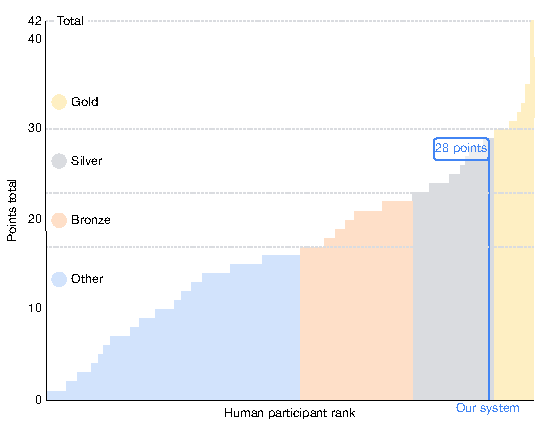
\includegraphics[width=0.75\linewidth]{../papers/translations/alphaproof/assets/fig5.pdf}\end{center}
\phantomsection
\noindent\textbf{原文图 5. 联合 AI 系统在 IMO 2024 的表现.}\paperlabel{5}{alphaproof-fig5}
联合系统得 28 分, AlphaProof 解三题 P1、P2、P6, AlphaGeometry 2\cite{alphaproof-ref3}解一题 P4. 相较人类参赛者\cite{alphaproof-ref27}, 该表现处于银牌区间. 图示官方金、银、铜牌分界. 图转载自文献\cite{alphaproof-ref28}, Google DeepMind.

\noindent\textbf{图中文字对应.} Total: 总分; Points total: 总得分; Gold、Silver、Bronze、Other: 金牌、银牌、铜牌、其他; Human participant rank: 人类参赛者排名; Our system: 我们的系统; 28 points: 28 分. 图中 42 分上限、奖牌边界与排名分布均保持原值.
